\documentclass[%
 aip,
amsmath,amssymb,
reprint,
]{revtex4-1}

\usepackage{graphicx}% Include figure files
\usepackage{dcolumn}% Align table columns on decimal point
\usepackage{bm}% bold math
\usepackage{verbatim}
\usepackage{subcaption}
%\usepackage[mathlines]{lineno}% Enable numbering of text and display math
%\linenumbers\relax % Commence numbering lines

\usepackage[utf8]{inputenc}
\usepackage[T1]{fontenc}
\usepackage{mathptmx}
\usepackage{etoolbox}
\usepackage{lipsum}


%% Apr 2021: AIP requests that the corresponding 
%% email to be moved after the affiliations
\makeatletter
\def\@email#1#2{%
 \endgroup
 \patchcmd{\titleblock@produce}
  {\frontmatter@RRAPformat}
  {\frontmatter@RRAPformat{\produce@RRAP{*#1\href{mailto:#2}{#2}}}\frontmatter@RRAPformat}
  {}{}
}%
\makeatother
\begin{document}

\preprint{AIP/123-QED}

\title[Intermediate Physics Laboratory 2, Module 2]{Tunable Differential Negative Resistor with an Operational Amplifier and N-Channel MOSFETs}
% Force line breaks with \\
\author{Myeong-gi Jo}
\altaffiliation{
whaudrl4005@gmail.com
}
\author{Subin Kim}
\altaffiliation{
subini0213@snu.ac.kr
}
\author{Jeong Min Lee}
\altaffiliation{
jmleeluck@snu.ac.kr
}
\author{Eugene Park}
\altaffiliation{
eupark@snu.ac.kr
}
\affiliation{ 
Department of Physics and Astronomy, Seoul National University
}

\date{\today}
\begin{abstract}
Negative resistors have shown multiple exotic physical phenomena in the electrical engineering field. This study presents an analysis of a negative resistor using an operational amplifier, with and without added n-channel MOSFETs. The negative differential resistance region is observed between a positive differential resistance region from $I-V$ characteristics. Various important properties of the negative differential resistor such as the differential resistance in the negative and positive region, negative differential resistance size, or the shape of the positive differential region have been changed by manipulating the resistance of a single resistor, operational amplifier supply voltage, and MOSFETs. A theoretical model explaining such modifications is introduced in line. This study demonstrates easily achievable methods of controlling several traits of a negative differential resistor, and other anomalous phenomena including hysteresis of the current.
\end{abstract}

\maketitle

\section{\label{sec:Intro} Introduction} 

For most standard electrical components, the relationship between applied voltage and current can be described to be linear. These ohmic devices are easily characterized by a straight current-voltage(\(I-V\)) curve. However, for non-linear devices, this \(I-V\) curve takes on a more complex shape, deviating from linearity. Within this domain of non-linear components, there emerges a fascinating phenomenon known as negative resistance. Unlike ordinary resistors, where the differential slope of the \(I-V\) curve is positive, negative resistance is characterized by certain intervals or regions in which an increase in voltage coincides with a decrease in current, causing the \(I-V\) curve to display this property. 

Such negative resistors have portrayed diverse physical phenomena, such as chaotic behavior in the Chua circuit\cite{chua_circuit,impact_chua}, Van der Pol oscillator\cite{VanDerPol}, and Negative Impedance Converters(NIC)\cite{NIC_BJT,NIC_MOSFET,NIC_MOSFET2}. In this paper, we design a negative resistor with and without MOSFETs, showing that the MOSFETs add higher non-linearity. We further provide descriptive experimentation and theoretical analysis of the $I-V$ curve characteristics, opening multiple tuning possibilities.\\


Operational amplifiers(Op--Amp) are a typical non--linear component that can amplify the difference between two voltage inputs. A realistic Op-Amp also saturates, which occurs when the output voltage of the Op--Amp reaches its maximum or minimum limit. In the case of an inverting Op--Amp, this leads to sudden positive current flow after a saturation point. This drives the motivation to start a design of a negative resistor using a feedback Op--Amp, which can allow positive differential resistance after a given voltage interval.
The ideal Op--Amp can be analyzed using three main rules.
\begin{itemize}
    \item Infinite Input Impedance : No current flows through the Op--Amp inputs.
    \item Zero Output Impedance : Current can be generated without limitation at the output of the Op--Amp
    \item Inverting and noninverting inputs of the Op--Amp have the same voltage.
\end{itemize}

Metal Oxide Semiconductor Field Effect Transistors(MOSFETs) are another interesting non--linear component. MOSFETs have only one type of charge carrier enabling easier to control terminals for operation. Operation of MOSFET has three regions characterized by the Gate--Source voltage($V_{\textrm{GS}}$) and Drain--Source voltage($V_{\textrm{DS}}$) as

\begin{itemize}
    \item Cut-off region ($V_{\textrm{GS}}<V_{\textrm{th}}$) : MOSFET is closed, and there will be no current flow through it. 
    \item Saturation region ($V_{\textrm{GS}}>V_{\textrm{th}}$, $V_{\textrm{DS}}>(V_{\textrm{GS}}-V_{\textrm{th}})$) : Current across the drain to source terminal will remain almost constant regardless of $V_{\textrm{DS}}$.
    \item Linear region ($V_{\textrm{GS}}>V_{\textrm{th}}$, $V_{\textrm{DS}}<(V_{\textrm{GS}}-V_{\textrm{th}})$) : Current across the drain to source terminal will linearly increase with $V_{\textrm{DS}}$.
\end{itemize}

\noindent where $V_{\textrm{th}}$ is threshold voltage. Thus MOSFET behaviors like a resistor in linear region. By short-circuiting the gate and source terminal, the MOSFET can be realized as a resistor that is voltage-gated. Combining this feature with the Op--Amp, an additional discontinuous slope to the $I-V$ characteristics can be obtained.\\

Using the theoretical characteristics of each nonlinear component, a theoretical model can be constructed to explain the negative differential resistance, and furthermore provide insight into tuning capabilities. Due to its complexity, the derivation and results will not be discussed in this section. For a detailed derivation of the $I-V$ characteristics, refer to the \textbf{Appendix}.\\


This report is organized as follows. In the Methods, we introduce our experimental method for designing and analyzing a non--linear resistor. The measurement data and $I-V$ characteristics of the negative resistor will be analyzed in Results. This includes the discussion of a discrepancy between measurement and theory, the effect of Op--Amp supply voltage, and hysteresis. The main findings and applications will be summarized in the Conclusion. Finally, in the Appendix a derivation of the theoretical analysis and the MOSFET characteristics will be demonstrated. 

\section{\label{sec:Method} Methods}

The negative resistor was designed with and without MOSFETs, and was measured with the circuit as in FIG. \ref{fig:Fig1} (a)\&(b), and the current was measured via a resistor $R$ in series in the negative resistor. The output voltage of the Op--Amp was also measured with respect to ground, to take into saturation of the Op--Amp in theoretical analysis. We sourced voltage from -5.0V to +5.0V in increasing increments of 0.1V, and then in reversed order. We repeated the measurement for $R=10\>\Omega,\>47\>\Omega,\>220\>\Omega,\>560\>\Omega,1120\>\Omega, 1680\>\Omega,1900\>\Omega,4700\>\Omega$. The values $R=10\>\Omega,\>47\>\Omega,\>220\>\Omega,\>560\>\Omega$ was mainly analyzed due to theoretical predictability. For the resistor values $R=560\>\Omega,1900\>\Omega$ the Op--Amp supply voltage was changed from $0$V to $5$V in $1$V increments to observe the effect of supply voltage to the negative differential resistance region. The values $R_{ref} = 1120\Omega, R_0 = 1k\Omega$ from FIG.\ref{fig:Fig1} (a)\&(b) were fixed for all of the experiments conducted.

An ADTL082J was used as the Op--Amp, and IRF1010E was used for the n-channel MOSFETs. Before the experimental process, the $I-V$ characteristics of the MOSFETs were measured in the circuit configuration to obtain a threshold voltage and the effective resistance when the MOSFET was open, with the circuit as in FIG. \ref{MOSFET_circuitfig}. The output voltage of the Op--Amp was also measured to compensate for the saturation effects of the real--world Op--Amp. We note that an unusual drop of current was observed near $V_0\sim-5V$. This seems to be caused by intrinsic Op--Amp characteristics and therefore was out of the scope of this research. Such regions have been omitted from the analysis.\\

As can be seen in FIG.\ref{fig:Fig1} (c)\&(d), the $I-V$ curve of the differential negative resistor can be divided into three regions with two distinguishable slopes and boundary points. In order to compare the differential resistance and the boundary points of each region with theoretically calculated ones, an algorithm that finds the boundary points and divided regions by detecting local maximal or minimal points of the $I-V$ curve was utilized. This is done by choosing the maximal or minimal point on the data array rather than regression of the graph near extremum points. In rare cases where the $I-V$ curve does not have an extremum point but two regions with significantly different slopes are distinguishable, we directly selected boundary points.

For each divided region, linear regression was conducted to obtain the differential resistance. For circuits with MOSFETs such as FIG. \ref{fig:Fig1} (d), the slope continuously changes for short regions at the end of the negative resistance region. Therefore, the outermost region with a constant slope was selected for the region of regression.


\section{\label{sec:Result} Results}

\subsection{Negative Resistance}
\begin{figure}[!h]
  \centering
  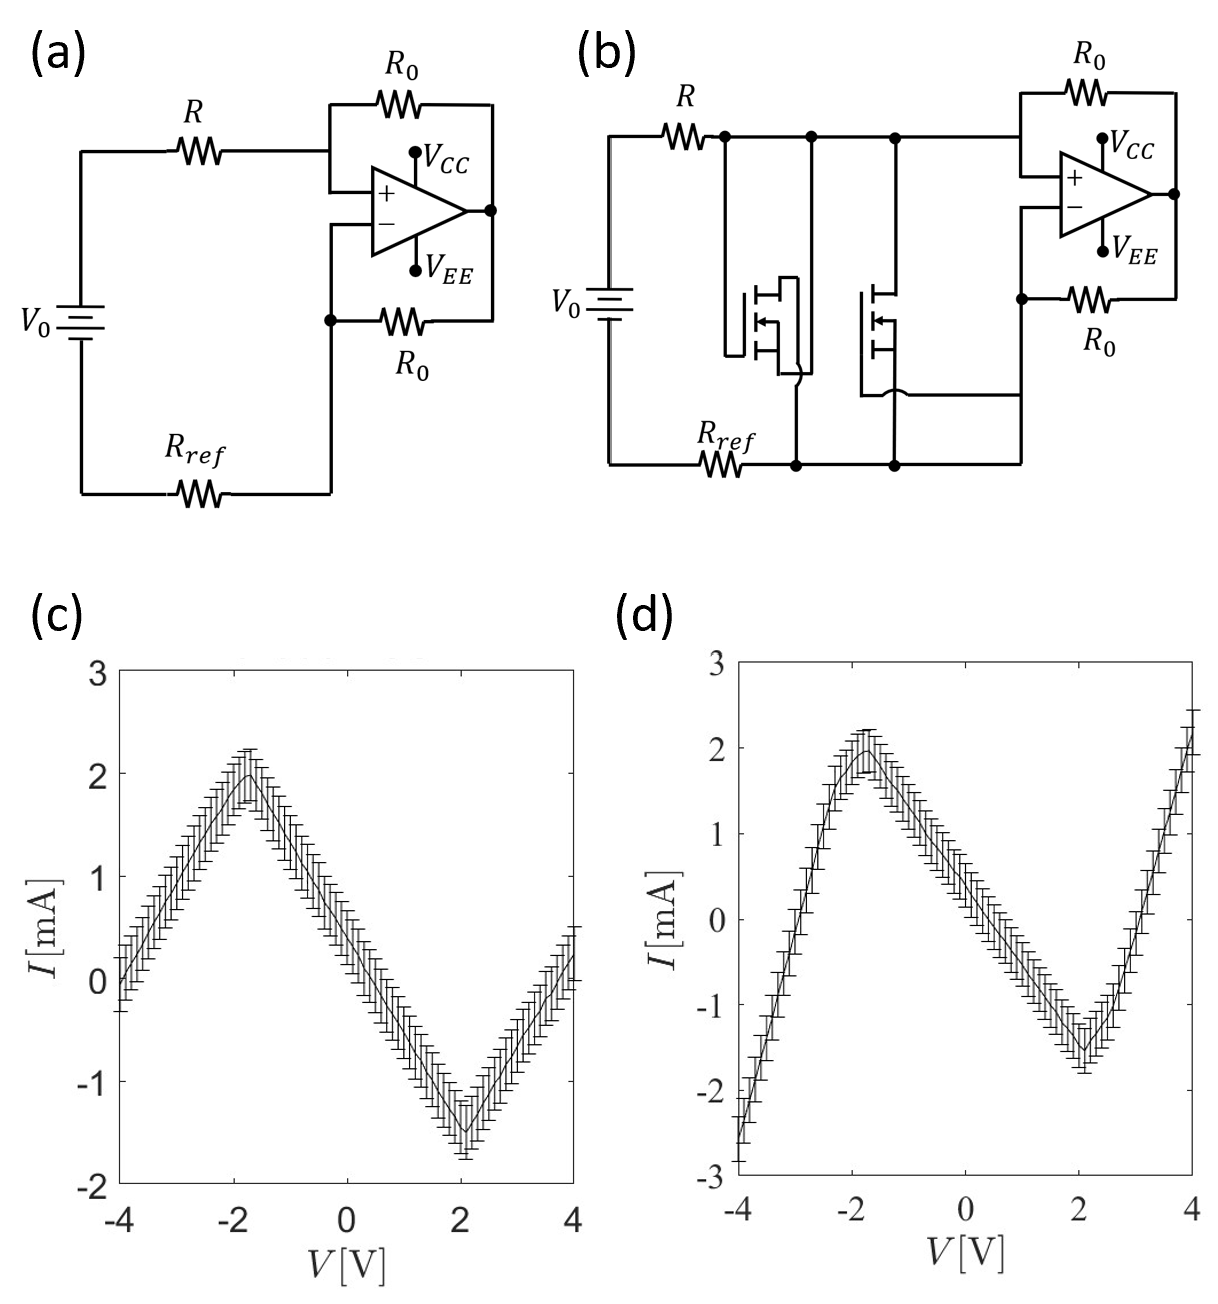
\includegraphics[width=0.45\textwidth]{figures/Fig1.png}
  \caption{(a) A schematic of the negative resistor circuit without MOSFETs (b) and with MOSFETs (c) The $I-V$ characteristics of the negative resistor without MOSFETs (d) and with MOSFETs. Regions I and II are depicted for clarity. Values of $R = 47\Omega, R_{ref} = 1120\Omega, R_0 = 1k\Omega$ were used for (c), (d)}
  \label{fig:Fig1}
\end{figure}

FIG.\ref{fig:Fig1} (a) is a schematic of an Op--Amp negative converter, and (b) is a schematic of the negative converter and MOSFETs connected parallel to the Op--Amp sub--circuit. The total current of the circuit with an applied voltage from -4V to 4V is depicted in FIG. \ref{fig:Fig1} (c) and (d) which is the $I-V$ curve used in the analysis. 

In region I, we successively observed the negative converter effect of Op--Amp to cause a negative differential resistance. The current is negative while the voltage across the circuit is positive, and vice versa. In region II, the slope gets positive rapidly due to the Op--Amp saturation. As the Op--Amp output is saturated, the output voltage does not change, and the system allows a voltage difference between the inverting and non--inverting inputs of the Op--Amp. This results in the invalidation of the negative converting effect.\\

The effect of MOSFETs in region I is negligible. For region II the positive slope of the $I-V$ curve is larger in the circuit with MOSFETs in region II, and an additional change of the slope after region I can be observed. This is because at region II of the circuit with MOSFETs the MOSFETs act as a voltage--gated switch with smaller resistance than the Op--Amp resistors. When the voltage across the MOSFETs exceeds its threshold the MOSFETs are activated. This increases the total flow of the circuit so that the slope of region II is larger with MOSFETs. The direct observation of the threshold voltage for the MOSFET voltage--gated switch can be seen through the voltage difference between the starting point of region II and the boundary point of region I. This region corresponds to the saturation of the Op--Amp with closed MOSFETs.\\

In addition to the $I-V$ characteristics, the output voltage of the Op--Amp is measured, and the saturation voltage is determined to be $V_{sat} = \pm 4.2121 \pm 0.0003 $V for a supply voltage of $V_G = 5$V. We estimated $V_{sat}$ by measuring the output voltage of Op--Amp. After the Op--Amp is saturated, the output voltage of the device is nearly constant. It was sufficient to get the saturated voltage by measuring the output voltage for input voltages larger than $4.5$V. The saturated voltage for several $R$ have been compared, and the sufficiently small standard error indicated an accurate $V_{sat}$.




\subsection{Tuning Differential Resistance Slopes}
The slope of the negative differential region and the positive region, including the extreme points($V_\text{in}^0$) of the $I-V$ characteristics are shown in FIG. \ref{fig:Fig2}.

\begin{figure}[!h]
  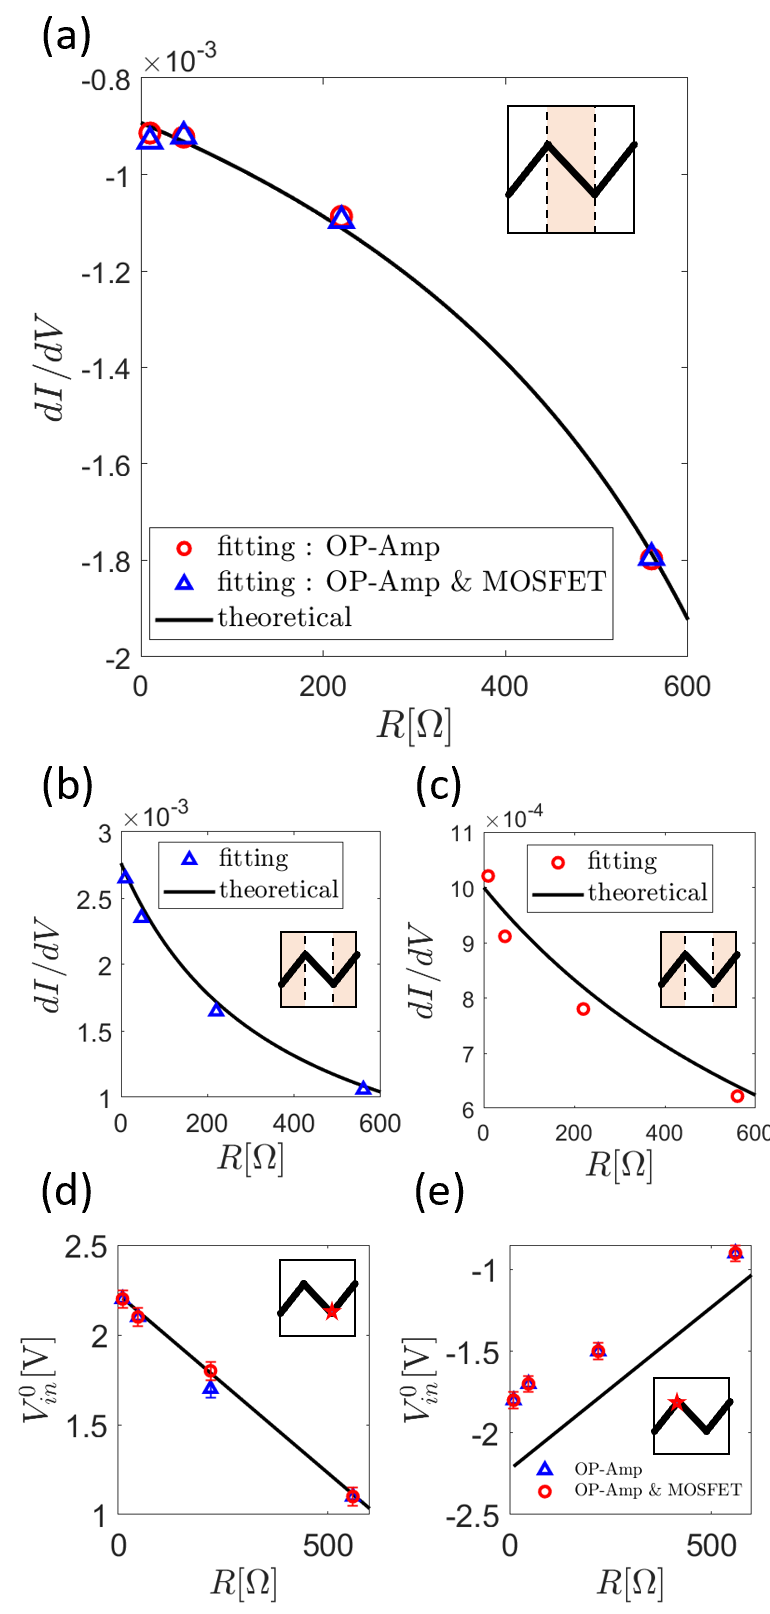
\includegraphics[width=0.45\textwidth]{figures/Fig2.png}
  \caption{The differential resistance of (a) region I, (b) region II for the Op--Amp and MOSFET negative resistor, (c) region II for the Op--Amp negative resistor, and the extreme points($V_\text{in}^{0}$) of both negative resistors having a (d) positive and (e) negative voltage value. The shaded region in the insets depicts the fitted region, and the red stars indicate the extreme value position relative to the $I-V$ curve. An Op--Amp supply voltage of $5$V was used. Error bars not visible are smaller than the marker.}
  \label{fig:Fig2}
\end{figure}

As can be seen, region I (FIG.\ref{fig:Fig2}. (a)) does not differ by the addition of MOSFETs and matches the theoretical value
\begin{eqnarray}
  i = -\frac{1}{R_{ref}-R}V_0
\end{eqnarray}
well for both negative resistors in the regime $R<R_{ref}$.

We further report on the discrepancy in the regime $R>R_{ref}$. According to theory, in this region, no negative differential resistance should be observed. However, experimental results have shown a negative resistance with a shift of the region I. This shift changes direction by the input voltage($V_0$) increment direction, leading to hysteresis. This has been observed for $R$ values up to $R=1900\Omega$, but for $R=4700\Omega$, the negative region disappears.

For region II, (FIG.\ref{fig:Fig2}. (b)\&(c)) the MOSFETs nearly double the slope. Both cases match the theory well, which gives the following values for the differential resistance.
\begin{widetext}
\begin{eqnarray}
  i_{MOSFET} = \frac{R_0R_{ref}+R_0R_m+R_mR_{ref}+R_0^2+R_{ref}R_0}{R_0^2(R_{ref}+R+R_m)+R_0(2R_{ref}R+R_{ref}R_m+R_mR)+R_mR_{ref}R}V_0 + \text{Intercept}\\
  i_{Op-Amp} = i^{ 0}+\frac{V_0-V_{sat}}{R+R_0}
\end{eqnarray}
\end{widetext}
The values $R,\,R_0,\,R_{ref},\,V_0$ are as in FIG.\ref{fig:Fig1} (a)\&(b), while $V_{sat}$ denotes the Op--Amp saturation voltage, and $i^0$ is the current flowing directly before saturation.\\

The extreme points($V_0^0$) show a linear dependence, for both cases. The positive extreme points(FIG.\ref{fig:Fig2}. (d)) match the theory as
\begin{equation}
    V_0^0 = V_{sat}\frac{R_{ref}-R}{R_{ref}+R_0}
\end{equation}
while the negative extreme points show a positive voltage shift(FIG.\ref{fig:Fig2}. (e)). We note that this discrepancy stems from the fact that the operating saturation voltage of the Op--Amp ADTL082J is not symmetrical, thus experimentally observed that the saturation occurs $\sim-3.5$V. This pushes the negative extreme points closer to $0$V. Despite this effect, the point for $V_0=0$ exhibits a negligible current flow $I\sim0.1$mA, excluding an unintended Op--Amp offset voltage as a possibility. \\

The higher slope of region II is due to the fact that the MOSFETs, acting as voltage gates, add another 'venting' channel for the current. Intuitively, the MOSFET effective resistor is smaller than $R_0$, thus decreasing the total resistance of the flowing current. The opposite effect can be obtained by adding high resistance resistors in series to each MOSFET and increasing the resistance of the flowing, thus decreasing the slope. Additionally, region I is indifferent to MOSFET addition since the current does not flow through MOSFETs in this region. By changing a single resistor of the negative resistor proposed, various values of negative differential resistance can be obtained and theoretically predicted with our model. The detailed derivation of the theoretical values is in the \textbf{Appendix}.

\subsection{Effect of Op--Amp Supply Voltage}
\begin{figure}[!h]
  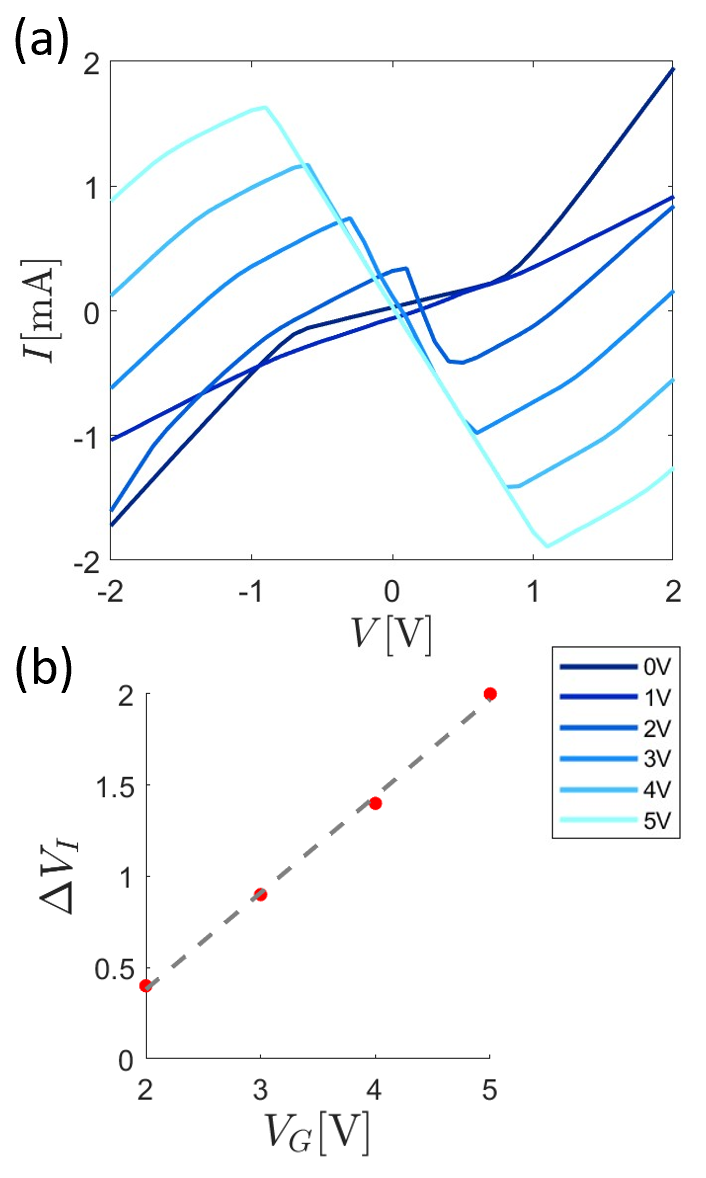
\includegraphics[width=0.45\textwidth]{figures/Fig3.png}
  \caption{(a) The $I-V$ curve by varying the Op--Amp supply voltage($V_G$).(b) The width of region I for different $V_G$ with a linear regression( $R^2=0.9979$). $R=560\Omega$ was used.}
  \label{fig:Fig3}
\end{figure}

By varying the supply voltage of Op--Amp, the region showing the negative resistance is getting broader. This can be verified by seeing FIG. \ref{fig:Fig3} (a). For 0V and 1V, the supply voltage is too small for negative resistance to appear. For the supply voltage greater or equal to 2V, the negative resistance starts to appear. The width of region I $\Delta V_I$ is calculated by subtracting the two boundary points. As can be seen in FIG.\ref{fig:Fig3} (b), the width of region I is strongly linear to the supply voltage. 

This linearity can be explained by referring to the features of Op--Amp.
For an ideal saturated Op--Amp, $V_{\text{sat}} = V_G$. Even though the Op--Amp that we used in this experiment is not ideal, still $V_{sat} \propto V_G$ for an extent. Thus, by noting that the boundary point for each $I-V$ curve is the moment when Op--Amp becomes saturated $V_0^0\propto V_{sat}$ holds. In total, $V_G \propto \Delta V_I = 2|V_0^0|$. This characteristic allows us to manipulate the width of the negative differential resistance region.


\subsection{Hysteresis Region}
\begin{figure}[!h]
  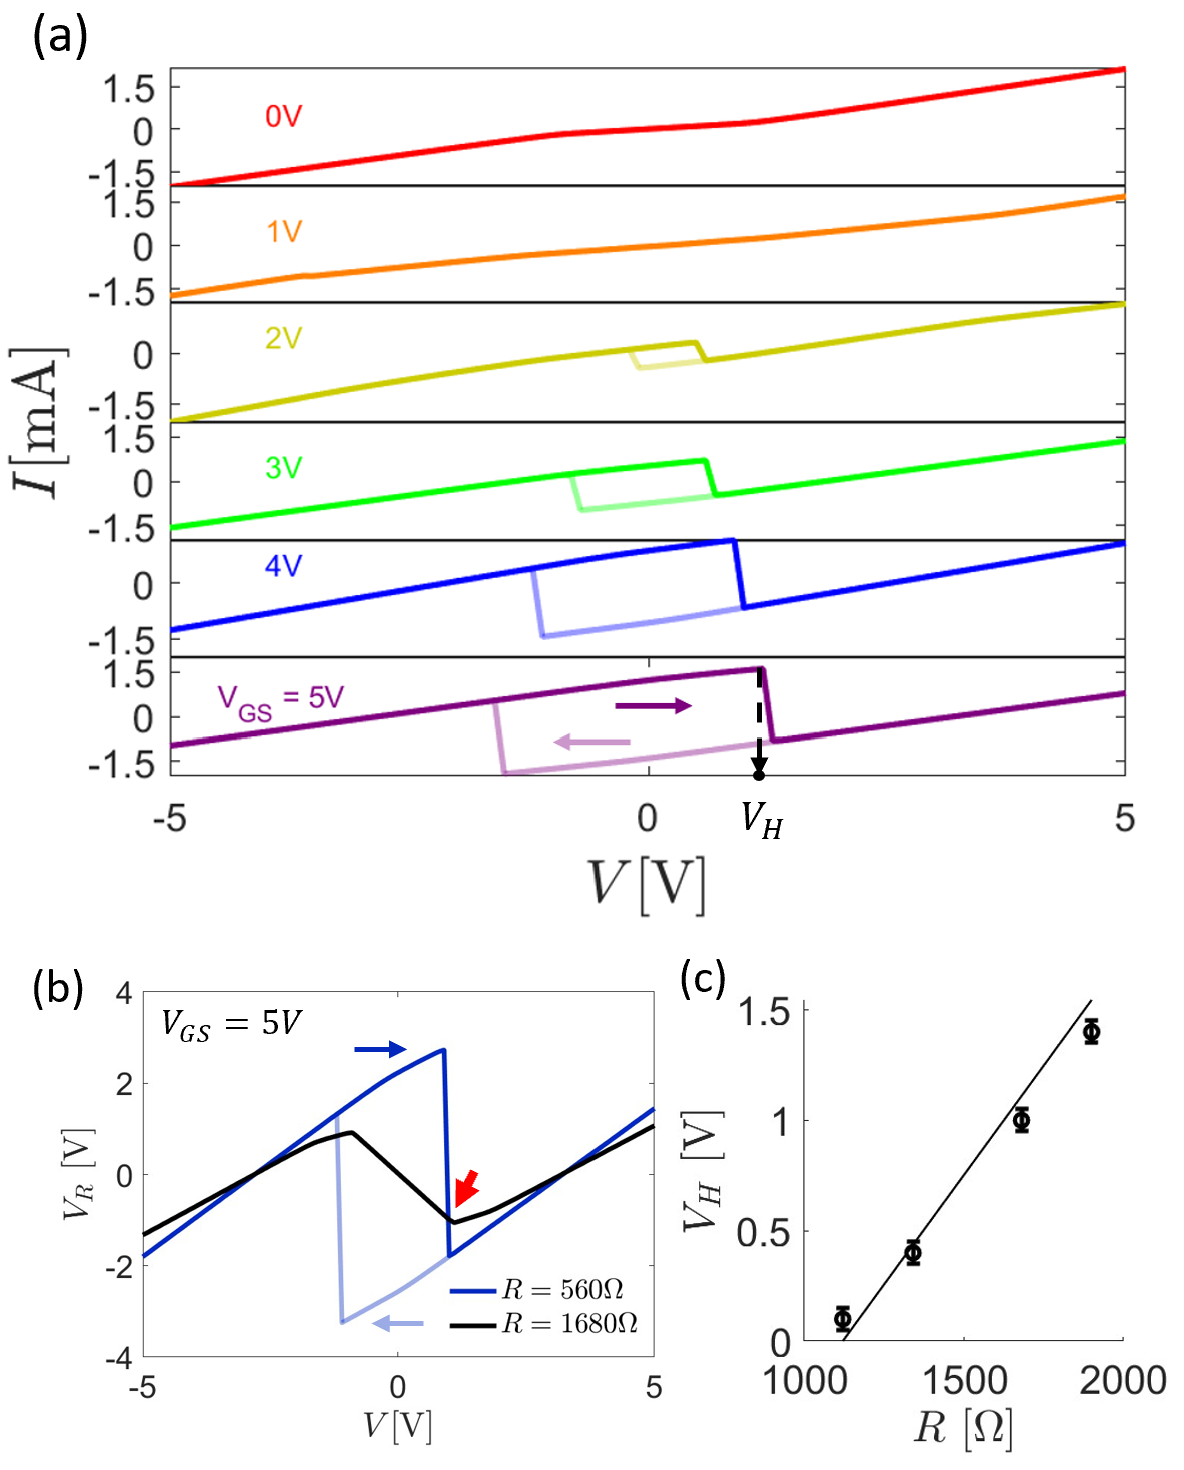
\includegraphics[width=0.48\textwidth]{figures/Fig4.png}
  \caption{(a) The $I-V$ curve of the negative resistor with Op--Amp and MOSFETs varying by different the supply voltage($V_{G}$). Hysteresis drop voltage $V_H$ is depicted. $V_H$. (b) The $I-V$ curves for $R = 560\Omega$, $R = 1680\Omega$. The value of the voltage drop through the resistor($R$) is used instead of current for easier comparison. The red arrow indicates the point $V_H$, which closely coincides with the extreme point when $R<R_{ref}$. (c) The value $V_H$ is fitted with region I boundary point value $|V_0^0|$.}
  \label{fig:Fig4}
\end{figure}

The negative resistor with Op--Amp and MOSFETs shows hysteresis behavior for a voltage ramp up and ramp down. The width of the hysteresis region changes by the Op--Amp supply voltage ($V_G$) and resistor ($R$) (FIG. \ref{fig:Fig1}). Especially, when considering an ideal operating situation of region I of the negative resistor, we observe that the boundary point of region I obtained by 
\begin{equation}
    V_0^0 = V_{sat}\frac{R_{ref}-R}{R_{ref}+R_0}
\end{equation}
has an absolute value of the hysteresis drop voltage $V_H$ (FIG.\ref{fig:Fig4}). This implies that the hysteresis is an artifact of the Op--Amp saturating, and thus cannot be observed in ideal working conditions. Therefore, these observations also open the possibility of tuning the width of the hysteresis loop using Op--Amp supply voltage($V_G$) and the resistor($R$) in the circuit. We underscore that such behavior is present even when changing the connections, the Op--Amp, the MOSFETs, and in conditions without the MOSFET, thus being an intrinsic effect of the Op--Amp in the operating configuration. 




\section{\label{sec:Conclusion} Conclusion}
We propose two negative resistors consisting of a single Op--Amp, with and without two MOSFETs. Using a theoretical model for the Op--Amp with added saturation effects, the negative differential resistance and region boundaries of the region I for both negative resistors can be modified to requirements. The addition of realistic saturation effects of the Op--Amp allows for theoretical prediction of the positive differential resistance of region II after saturation. The of addition another differential resistance after the boundary of region I and the differential resistance far of region II can be altered by using MOSFETs as a voltage-gated switch, which means MOSFETs can be used to tune positive region slope while unchanging negative converting region. 

Furthermore, the supply voltage of the Op--Amp is also a viable route for tuning the $I-V$ characteristics. This methodology opens corners for tuning differential negative resistance, and also designing non-linear effects for the Op--Amp saturated region. Some discrepancy between the experimental negative boundary of the region I and the theory can be attributed to the asymmetrical effect of the Op--Amp. Such realistic terms can be further added to the theoretical model to increase accuracy.\\

Hysteresis for values $R>R_{ref}$ has also been observed. Regarding the reproducibility of the effect, it is considered as an intrinsic effect of the Op--Amp. Such emergent properties offer opportunities for diverse physical phenomena with simple elements. \\

Due to the nonlinear characteristics, the negative resistor proposed is expected to show nonlinear features that are different from other well--known systems, such as the Chua circuit\cite{chua_circuit} differs in region I and the Van der Pol oscillator\cite{VanDerPol} differs in the fact that the $I-V$ curve has abrupt slope changes. The negative resistor can possibly exhibit a new type of Lienard equation, which will be further discussed in future work. 



\appendix

\section{\label{mosfetiv}MOSFET $I-V$ Characteristics}


\begin{figure}[!htbp]
  \begin{subfigure}{0.15\textwidth}
    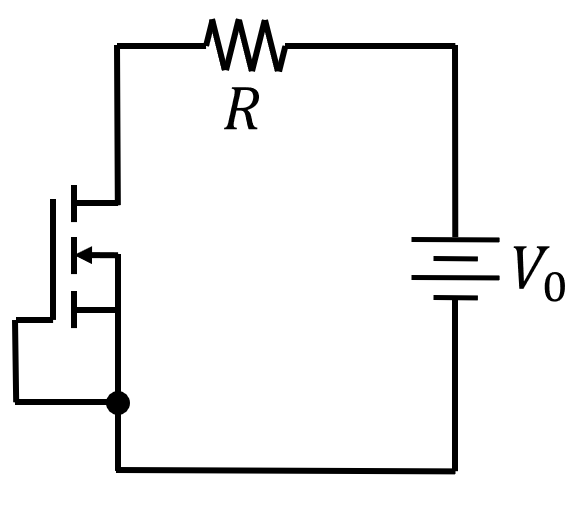
\includegraphics[width=\linewidth]{figures/MOSFET_circuit.png}
    \caption{}
    \label{MOSFET_circuitfig_a}
  \end{subfigure}%
  %\hspace*{\fill}   % maximize separation between the subfigures
  \begin{subfigure}{0.23\textwidth}
    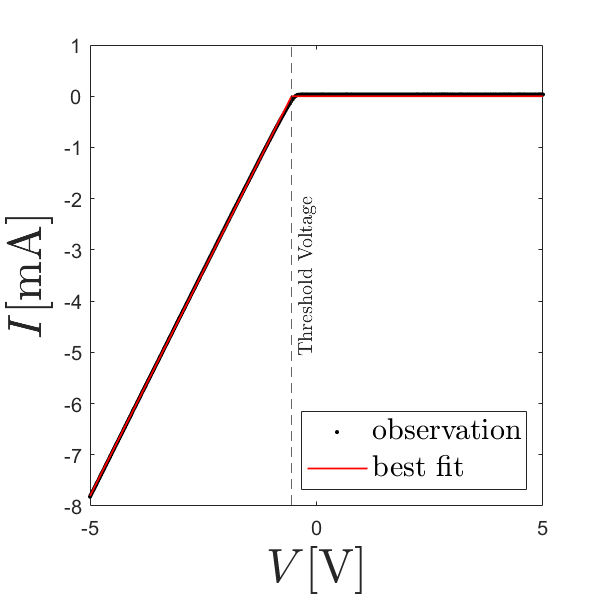
\includegraphics[width=\linewidth]{figures/MOSFETIV.png}
    \caption{}
    \label{MOSFET_circuitfig_b}
  \end{subfigure}

\caption{(a) A schematic setup for testing MOSFET $I-V$ characteristic. (b) Experimental result of MOSFET $I-V$ characteristic. Black dots show experiment data and the red line is the best fit to (\ref{MOSFET_eq}). The threshold voltage is denoted as a dashed line.} \label{MOSFET_circuitfig}
\end{figure}

In this experiment, two MOSFETs with a gate terminal and a source terminal connected to each other are used.
The MOSFET is open when the gate--source voltage is higher than the threshold voltage, and current through MOSFET linearly increases as gate--drain voltage increases.
This property can be characterized as 

\begin{equation}
I=\frac{V-V_{\textrm{th}}}{(R+R_{\textrm{m}})}\theta(V-V_{\textrm{th}})
\label{MOSFET_eq}
\end{equation}

\noindent where $V_{\textrm{th}}$ is threshold voltage, $R_{\textrm{m}}$ is effective resistance of MOSFET, and $\theta(V)$ is Heaviside step function.
To test this $I-V$ characteristic, we set the circuit as FIG. \ref{MOSFET_circuitfig_a}.
Voltage was sourced from -5.00V to +5.00V in increments of 0.1V, with a resistor of $R=560\Omega$.

The result is plotted in FIG.\ref{MOSFET_circuitfig_b}, where experimental data is denoted as black dots, best fit to (\ref{MOSFET_eq}) as a red line, and threshold voltage as a dashed line.
Note that the gate--drain voltage is negative when $V_{0}>0$ and vice versa in this setup, so we put $(V-V_{\textrm{th}})\rightarrow-(V-V_{\textrm{th}})$ and $I\rightarrow -I$ into the equation.
Our best fit values are $V_{\textrm{th}}=0.5505\pm0.0015$ V and $R_{\textrm{m}}=10.21\pm0.33\>\Omega$.


\section{Derivation of the theoretical $I-V$ Characteristics of the Negative Resistor}

\begin{figure}[!h]
  \centering
  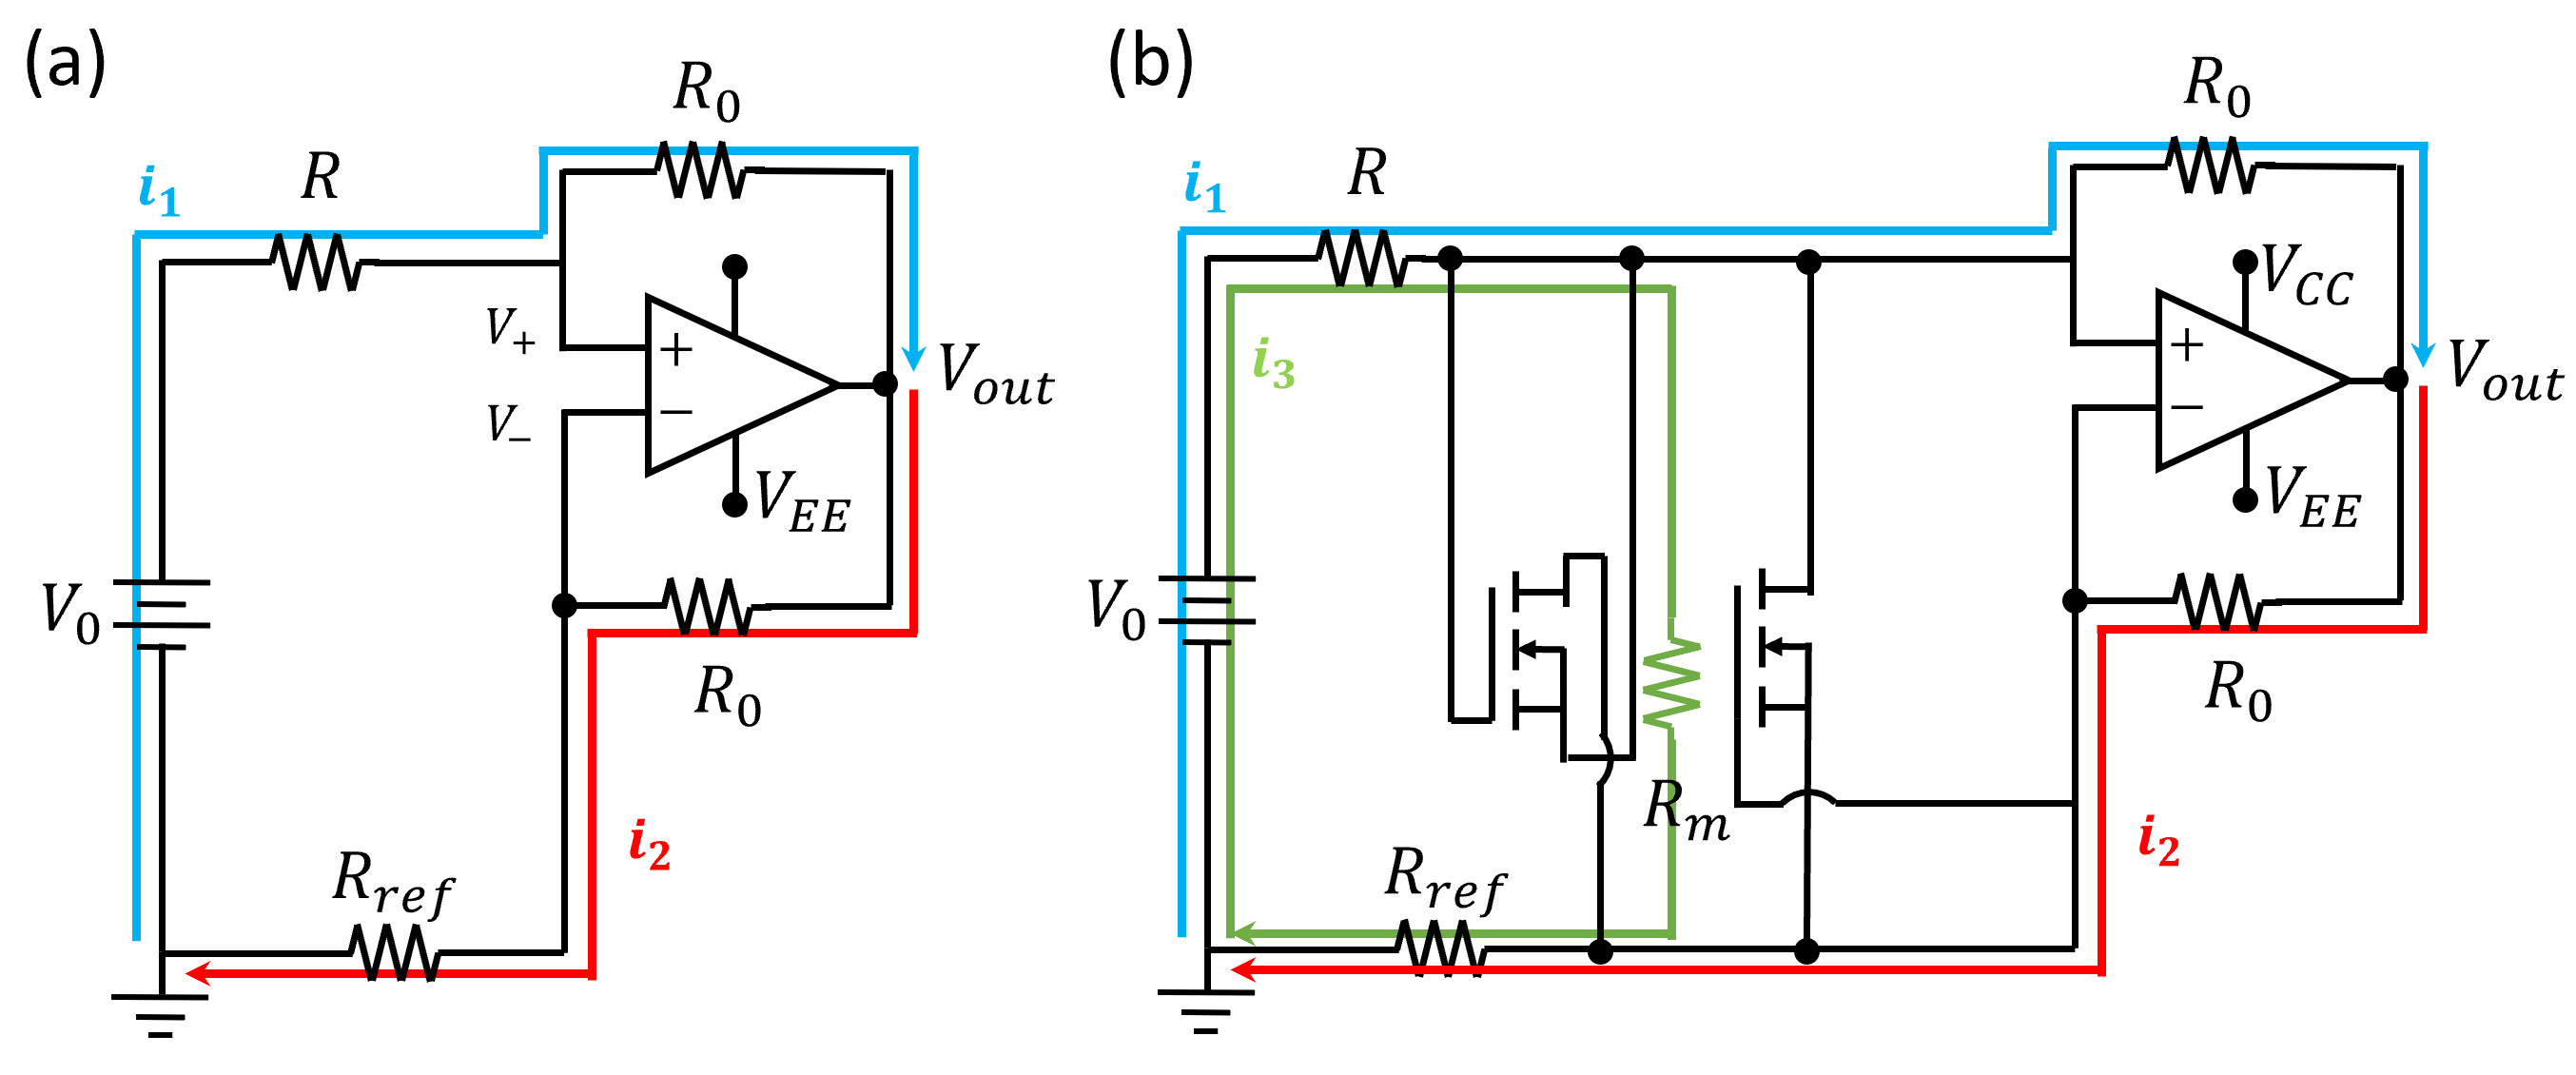
\includegraphics[width=0.45\textwidth]{figures/Appendix2.png}
  \caption{The currents flowing when operated for the negative differential resistor (a) without MOSFETs and (b) with MOSFETs.}
  \label{fig:OpAmpTheory}
\end{figure}

\subsubsection{\label{opampiv}Op--Amp Negative Resistor}
For the negative resistor with only an Op--Amp, an ideal op amp is assumed for the theoretical calculation of the unsaturated region. Therefore, the input voltage of the inverting and non-inverting inputs of the Op--Amp are identical($V_+=V_-$). Using this fact, following FIG.\ref{fig:OpAmpTheory} the following equations are obtained.
\begin{eqnarray}
  V_0-Ri_1 = V_+\\
  V_+ -R_0i_1 = V_{out}\\
  V_{out}-R_0i_2=V_-\\
  V_--R_{ref}i_2=0\\
  V_+ = V_-
\end{eqnarray}
By solving these $5$ equations, the following results can be obtained.
\begin{eqnarray}
  V_{out} = \frac{R_{ref}+R_0}{R_{ref}-R}V_0\\
  i_1 = -\frac{1}{R_{ref}-R}V_0
\end{eqnarray}

For the saturated region, we note that the saturated voltage is held constant as $V_{out} = V_{sat}$. Then the following equations can be obtained, assuming the surplus current created after the turning point of region I all enters to the output end of the Op--Amp. Note that the assumption of the infinite impedance of the Op--Amp is still kept. Thus, the following equation can be constructed,
\begin{equation}
    V_{0} -i(R+R_0) = V_{sat}
\end{equation}
giving the total following current $i$ as the following, where $i^0$ is the current at the boundary point of region I.
\begin{equation}
    i = i^0+\frac{V_0-V_{sat}}{R+R_0}
\end{equation}


\subsubsection{\label{opamp_mosfetiv}Op--Amp and MOSFETs Negative Resistor}
The unsaturated region of the negative resistor using enabling MOSFETs is identical to the unsaturated region of the negative resistor without the MOSFETs since all of the MOSFETs do not flow current. We derive a theoretical description of the differential resistance slopes for the region where a MOSFET is opened. 

The three currents present after saturation are depicted in FIG.\ref{fig:OpAmpTheory} (b). In the saturated state, the output voltage of the Op--Amp is fixed as $V_{out}-V_{sat}$. Using this fact, the following three equations are obtained.

\begin{eqnarray}
  V_{sat} = V_0-R(i_1+i_2)-i_1R_0\\
  V_0 - R(i_1+i_2)-R_mi_2-R_{ref}(i_2+i_3) = 0\\
  V_{sat} -i_3R_0-(i_2+i_3)R_{ref} = 0\\
\end{eqnarray}

When solving the previous equations, a solution we can obtain is the following:
\begin{widetext}
\begin{eqnarray}
  i_1 = \frac{V_{sat}(-R_0R_{ref}-R_0R-R_mR_0-R_mR_{ref})+V_0(R_0R_{ref}+R_mR_0+R_mR_{ref})}{R_0^2R_{ref}+R_0^2R+R_mR_0^2+2R_0R_{ref}R+R_mR_0R_{ref}+R_mR_0R+R_mR_{ref}R}\\
  i_2 = \frac{R_0(V_{sat}(-R_{ref}+R)+V_0(R_0+R_{ref}))}{R_0^2R_{ref}+R_0^2R+R_mR_0^2+2R_0R_{ref}R+R_mR_0R_{ref}+R_mR_0R+R_mR_{ref}R}\\
  i_3 = \frac{V_{sat}(R_0R_{ref}+R_0R+R_mR_0+R_mR)-V_0R_0R_{ref}}{R_0^2R_{ref}+R_0^2R+R_mR_0^2+2R_0R_{ref}R+R_mR_0R_{ref}+R_mR_0R+R_mR_{ref}R}
\end{eqnarray}
\end{widetext}
The current flowing through $R$ is $i_1+i_2$, thus giving the proportional constant to $V_0$ as the following:
\begin{widetext}
\begin{equation}
  i_1+i_2 = \frac{R_0R_{ref}+R_0R_m+R_mR_{ref}+R_0^2+R_{ref}R_0}{R_0^2(R_{ref}+R+R_m)+R_0(2R_{ref}R+R_{ref}R_m+R_mR)+R_mR_{ref}R}V_0 + \text{Intercept}
\end{equation}
\end{widetext}

\bibliographystyle{unsrt}
\bibliography{references}
\end{document}
